\section{Analisi degli errori}
Parliamo ora delle tecniche per l'analisi dell'errore. La continuità della funzione implica che il problema sia
\emph{ben posto}. Dalla relazione
\[
	\ein = \frac{f(\tx) - f(x)}{f(x)} =
	\frac{f(\tx) - f(x)}{\tx - x} \frac{x}{f(x)} \frac{\tx - x}{x}
\]
si ricava che la \emph{differenziabilità} di $f(x)$ è essenziale per il controllo dell'errore inerente. In
particolare se la funzione è \textbf{regolare}, ossia derivabile volte con derivate continue, allora vale
lo sviluppo di Taylor
\[ f(\tx) = f(x) + f'(x) (\tx - x) + \frac{f''(\xi) \cdot (\tx - x)^2}{2} \]
con $|\xi - x| \leq |\tx - x|$, da cui si ottiene
\[
	\ein = \frac{f(\tx) - f(x)}{f(x)} \doteq \frac{f'(x)}{f(x)} \cdot x \cdot \epsilon_x
	= c_x \cdot \epsilon_x
\]

\subsection{Coefficiente di amplificazione}
\begin{definition}
	La quantità
	\[ c_x = c_x (f) = \frac{f'(x)}{f(x)} \cdot x \]
	è detta \textbf{coefficiente di amplificazione} e fornisce una misura del condizionamento del problema.
\end{definition}

Più in generale possiamo dire che se $f : \Omega \to \R$ è definita su un insieme aperto di $\R^n$, differenziabile
due volte su $\Omega$ ed il segmento di estremi $\tx$ e $x$ è contenuto in $\Omega$ allora vale
\[
	\ein = \frac{f(\tx) - f(x)}{f(x)} \doteq
	\frac{1}{f(x)} \sum_{i=1}^n \frac{\partial f}{\partial x_i} (x) x_i \epsilon_{x_i} =
	\sum_{i=1}^n c_{x_i} (f) \epsilon_{x_i}
\]
con
\[ c_{x_i} (f) = \frac{1}{f(x)} \frac{\partial f}{\partial x_i} (x) x_i \]
con $1 \leq i \leq n$, detti coefficienti di amplificazione della funzione $f$ rispetto alla variabile $x_i$.

\begin{example}
	Per $f(x) = \frac{x^2 + 1}{x}$ si ha
	\[
		c_x = \left( 2 - \frac{x^2 + 1}{x^2} \right) \cdot \frac{x}{x^2 + 1} \cdot x =
		\frac{x^2 - 1}{x^2 + 1}
	\]
	Poiché $|c_x| \leq 1$ il problema del calcolo di $f(x)$ risulta ben condizionato.
\end{example}

\begin{example}
	Studiamo il condizionamento di $f(x, y) = x - y$, ossia studiamo l'errore inerente. Per farlo, calcoliamo
	\[ f(\tx, \tilde{y}) = \tx - \tilde{y} = x \cdot (1 + \epsilon_x) - y \cdot (1 + \epsilon_y) \]
	che equivale a
	\[ f(x, y) + x \epsilon_x - y \epsilon_y \]
	Se proviamo a calcolare l'errore inerente otteniamo
	\[
		\ein = \frac{f(\tx, \tilde{y}) - f(x, y)}{f(x, y)} =
		\frac{x}{x - y} \cdot \epsilon_x - \frac{y}{x - y} \cdot \epsilon_y
	\]
	Per terminare possiamo dire che il problema è mal condizionato per valori vicini di $x$ e $y$ con segno
	concorde.
\end{example}

\begin{example}
	Studiamo il condizionamento di $f(x, y) = x\cdot y$
	\[
		f(\tx, \tilde{y}) = \tx \cdot \tilde{y} = x (1 + \epsilon_x) \cdot y (1 + \epsilon_y) =
		f(x, y) \cdot (1 + \epsilon_x + \epsilon_y)
	\]
	Ne segue che l'errore inerente ha valore
	\[ \ein = \frac{f(\tx, \tilde{y}) - f(x, y)}{f(x, y)} = \epsilon_x + \epsilon_y \]
	che, come possiamo notare, ha un coefficiente di amplificazione costante.
\end{example}

\subsubsection{Cancellazione numerica}
Come possiamo notare, l'errore inerente, nel caso della sottrazione (ma anche addizione) di numeri vicini fra
loro tende ad essere amplificato molto, causando così il fenomeno di \textbf{cancellazione numerica}, portando
cosiddetti \textbf{errori di cancellazione}. Supponiamo di volere calcolare la differenza tra due numeri $x$
e $y$
\begin{align*}
	x = & 0. d_1 \dots d_i d_{i+1} \dots d_t \\
	y = & 0. d_1 \dots d_i d_{i+1} \dots d_t
\end{align*}
dove le prime $i$ cifre sono uguali. Supponiamo che queste due quantità abbiano del rumore sulle ultime cifre.
Quando viene effettuata la sottrazione le prime $i$ cifre si annullano e le ultile cifre, dato che siamo in
virgola mobile, vengono portate in testa. Abbiamo quindi portato il rumore in testa di conseguenza.

Per le operazioni moltiplicative invece la situazione cambia e al contrario di quanto si possa pensare, i problemi
moltiplicativi sono, in generale, ben condizionati.

\subsection{Calcolo dell'errore algoritmico mediante grafi}
Supponiamo di avere un algoritmo di calcolo di questo tipo
\begin{lstlisting}[language=pseudo]
...
...
z = x + y
...
...
\end{lstlisting}
Quello che verrà calcolato in macchina sarà
\[ \hat{z} = \hat{x} \oplus \hat{y} \]
dove $\hat{x} = x (1 + \epsilon)$ e $\hat{y} = y (1 + \delta)$. I due errori $\epsilon$ e $\delta$ non sono gli
errori di rappresentazione di $x$ e $y$ ma tutto l'errore accumulato fino a quel momento nel calcolo di $x$ e $y$.
Da qui possiamo calcolare $\hat{z}$ come segue
\begin{align*}
	\hat{z} = & [ x (1 + \epsilon) + y (1 + \delta) ] (1 + \epsilon_1) \quad |\epsilon_1| \leq u \\
	=         & x (1 + \epsilon + \epsilon_1) + y (1 + \delta + \epsilon_1)
\end{align*}
Calcoliamo ora l'errore accumulato su $\hat{z}$
\[ \etot = \frac{\hat{z} - z}{z} = \frac{x}{x + y} \epsilon + \frac{y}{x + y} \delta + \epsilon_1 = \eta \]
Ne concludiamo che l'errore accumulato su $z$ dipende dall'errore locale dell'operazione e dagli errori presenti
sugli operandi, amplificati dai coefficienti di amplificazione dell'operazione che stiamo considerando (in questo
caso la somma). Graficamente possiamo rappresentare la situazione in questo modo
\begin{center}
	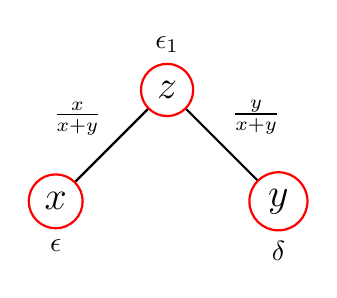
\begin{tikzpicture}[node distance=2cm, mynode/.style={draw=red, thick, circle, font=\Large}]
		\node[mynode, label=above:$\epsilon_1$] (1) {$z$};
		\node[mynode, below left of=1, label=below:$\epsilon$] (2) {$x$};
		\node[mynode, below right of=1, label=below:$\delta$] (3) {$y$};

		\path
		(1) edge[thick] node[above left, black] {$\frac{x}{x+y}$} (2)
		(1) edge[thick] node[above right, black] {$\frac{y}{x+y}$} (3);
	\end{tikzpicture}
\end{center}

\subsubsection{Analisi all'indietro}
In un'\textbf{analisi all'indietro} si assume che i dati in ingresso siano numeri di macchina e che quindi non
abbiano errori di rappresentazione. Si assume di conseguenza che il valore effettivamente calcolato non sia
$g(\tx)$ ma $f(\hat{x})$, ossia che il valore $g(\tx)$ risulti uguale, in un'analisi al primo ordine, al valore
assunto dalla funzione esatta $f$ valutata in un dato perturbato $\hat{x}$. Queste assunzioni implicano un errore
di rappresentazione \textbf{nullo} sui dati in ingresso.

\begin{example}
	Proviamo a trattare in questo modo due algoritmi già visti in precendenza. Vogliamo valutare la stabilità
	di $\frac{x - 1}{x}$ e $1 - \frac{1}{x}$. Nel primo caso, il grafo avrà questo aspetto
	\begin{center}
		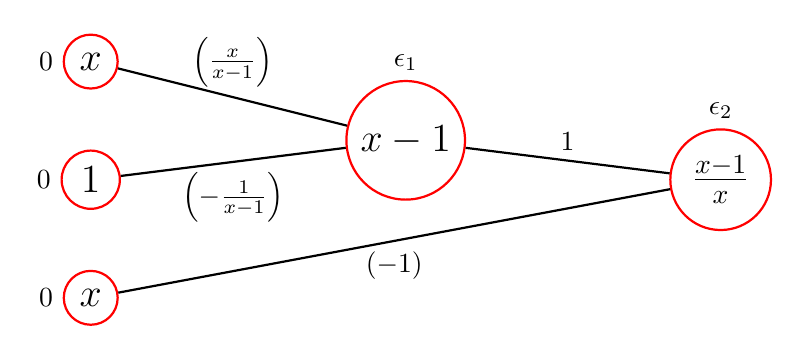
\begin{tikzpicture}[mynode/.style={draw=red, thick, circle, font=\Large}]
			\node[mynode, label=left:$0$] at (0, 1.5) (x1) {$x$};
			\node[mynode, label=left:$0$] at (0, 0) (1) {$1$};
			\node[mynode, label=left:$0$] at (0, -1.5) (x2) {$x$};

			\node[mynode, label=above:$\epsilon_1$] at (4, 0.5) (x-1) {$x-1$};
			\node[mynode, label=above:$\epsilon_2$] at (8, 0) (x-1/x) {$\frac{x-1}{x}$};

			\path
			(x1) edge[thick] node[above, black] {$\left( \frac{x}{x-1} \right)$} (x-1)
			(1) edge[thick] node[below, black] {$\left( -\frac{1}{x-1} \right)$} (x-1)
			(x-1) edge[thick] node[above, black] {$1$} (x-1/x)
			(x2) edge[thick] node[below, black] {$(-1)$} (x-1/x);
		\end{tikzpicture}
	\end{center}
	Dato che stiamo calcolando l'errore algoritmico non mettiamo errore sui dati in ingresso, poiché assumiamo
	che essi siano numeri di macchina (possiamo mettere 0 se preferiamo).

	Fatta questa considerazione diventa inutile anche scrivere i coefficienti di amplificazione dovuti
	alle operazioni di sottrazione e divisione (per quanto riguarda il denominatore) in quanto verrebbero
	moltiplicati per 0.

	L'unico coefficiente di amplificazione che ha senso scrivere è quello dovuto all'operazione di divisione (per
	quanto riguarda il numeratore) in quanto andrebbe a moltiplicare l'errore locale $\epsilon_1$ dovuto
	all'operazione di sottrazione.

	Terminiamo scrivendo l'errore locale $\epsilon_2$ dovuto all'operazione di divisione sull'ultimo nodo. L'errore
	algoritmico si ricava sommando tutti i prodotti tra i nodi e i coefficienti di amplificazione posti sugli archi
	adiacenti a tali nodi.
	\begin{align*}
		\ealg =   & 0 \cdot \frac{x}{x-1} + 0 \cdot \left( -\frac{1}{x-1} \right) + 0 \cdot (-1) +
		\epsilon_1 \cdot 1 + \epsilon_2                                                            \\
		=         & \epsilon_1 + \epsilon_2                                                        \\
		\\
		|\ealg| = & |\epsilon_1| + |\epsilon_2| \leq 2u
	\end{align*}
	ovvero il risultato ottenuto dall'analisi già fatta in precendenza. Dato che i coefficienti di amplificazione
	che moltiplicano errori non nulli sono costanti, possiamo concludere che l'algoritmo sia numericamente stabile.

	Disegnamo il grafo anche per l'algoritmo $1 - \frac{1}{x}$, senza spiegare nuovamente tutti i passaggi
	\begin{center}
		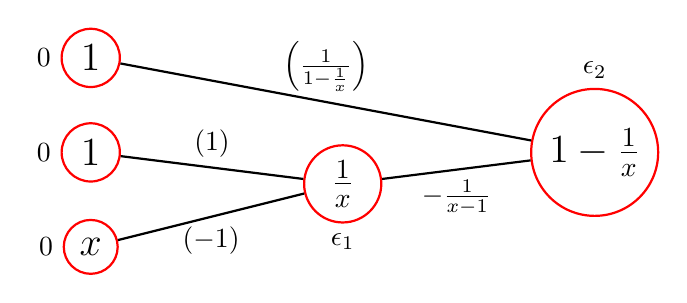
\begin{tikzpicture}[scale=0.8, mynode/.style={draw=red, thick, circle, font=\Large}]
			\node[mynode, label=left:$0$] at (0, 1.5) (11) {$1$};
			\node[mynode, label=left:$0$] at (0, 0) (12) {$1$};
			\node[mynode, label=left:$0$] at (0, -1.5) (x) {$x$};

			\node[mynode, label=below:$\epsilon_1$] at (4, -0.5) (1/x) {$\frac{1}{x}$};
			\node[mynode, label=above:$\epsilon_2$] at (8, 0) (1-1/x) {$1 - \frac{1}{x}$};

			\path
			(11) edge[thick] node[above, black] {$\left( \frac{1}{1 - \frac{1}{x}} \right)$} (1-1/x)
			(12) edge[thick] node[above, black] {$(1)$} (1/x)
			(x) edge[thick] node[below, black] {$(-1)$} (1/x)
			(1/x) edge[thick] node[below, black] {$-\frac{1}{x-1}$} (1-1/x);
		\end{tikzpicture}
	\end{center}
	In questo caso, l'errore algoritmico risulta
	\begin{align*}
		\ealg =   & 0 \cdot \frac{1}{1 - \frac{1}{x}} + 0 \cdot 1 + 0 \cdot (-1) +
		\epsilon_1 \cdot \left( -\frac{1}{x-1} \right) + \epsilon_2                                    \\
		=         & -\frac{1}{x-1} \cdot \epsilon_1 + \epsilon_2                                       \\
		\\
		|\ealg| = & \frac{1}{|x-1|} \cdot |\epsilon_1| + |\epsilon_2| \leq \frac{1}{|x-1|} \cdot u + u
	\end{align*}
	Ne deduciamo che per valori di $x$ prossimi a 1 l'algoritmo è numericamente instabile.
\end{example}
Come possiamo notare, un'analisi all'indietro conduce a risultati più ottimistici e spesso anche più realistici
per una buona valutazione dell'errore algoritmico.

\subsubsection{Analisi in avanti}
L'\textbf{analisi in avanti} è di norma più pessimista in quanto considera il massimo errore accumulabile e quindi
considera anche l'errore di rappresentazione dei dati in ingresso. Vediamo come cambiano il grafo e dunque il
calcolo dell'errore per l'algoritmo $\frac{x-1}{x}$.
\begin{center}
	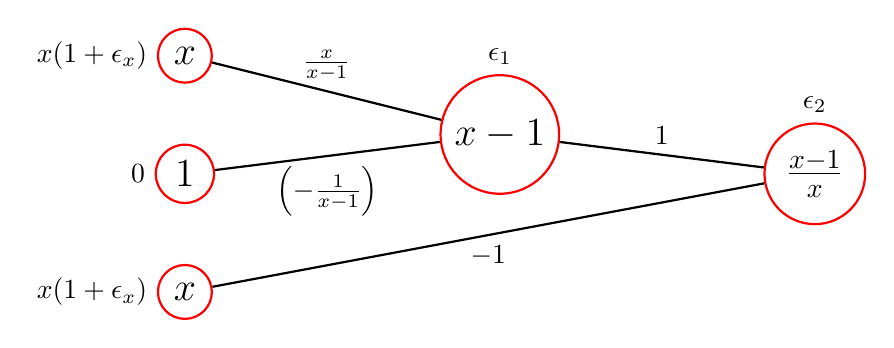
\begin{tikzpicture}[mynode/.style={draw=red, thick, circle, font=\Large}]
		\node[mynode, label=left:$x(1 + \epsilon_x)$] at (0, 1.5) (x1) {$x$};
		\node[mynode, label=left:$0$] at (0, 0) (1) {$1$};
		\node[mynode, label=left:$x(1 + \epsilon_x)$] at (0, -1.5) (x2) {$x$};

		\node[mynode, label=above:$\epsilon_1$] at (4, 0.5) (x-1) {$x-1$};
		\node[mynode, label=above:$\epsilon_2$] at (8, 0) (x-1/x) {$\frac{x-1}{x}$};

		\path
		(x1) edge[thick] node[above, black] {$\frac{x}{x-1}$} (x-1)
		(1) edge[thick] node[below, black] {$\left( -\frac{1}{x-1} \right)$} (x-1)
		(x-1) edge[thick] node[above, black] {$1$} (x-1/x)
		(x2) edge[thick] node[below, black] {$-1$} (x-1/x);
	\end{tikzpicture}
\end{center}
In questo caso abbiamo
\begin{align*}
	g(\tx) = & x (1 + \epsilon_x) \frac{x}{x-1} - x (1 + \epsilon_x) + \epsilon_1 + \epsilon_2 \\
	=        & x (1 + \epsilon_x) \left( \frac{x}{x-1} - 1 \right) + \epsilon_1 + \epsilon_2   \\
	=        & (1 + \epsilon_x) \left( \frac{x}{x - 1} \right) + \epsilon_1 + \epsilon_2       \\
	=        & \frac{x}{x - 1} + \frac{x}{x-1} \epsilon_x + \epsilon_1 + \epsilon_2
\end{align*}